% !TEX TS-program = pdflatex
% !TEX encoding = UTF-8 Unicode

% This is a simple template for a LaTeX document using the "article" class.
% See "book", "report", "letter" for other types of document.

\documentclass[11pt]{article} % use larger type; default would be 10pt

\usepackage[utf8]{inputenc} % set input encoding (not needed with XeLaTeX)
\usepackage{lscape,amsmath,amssymb}
%%% Examples of Article customizations
% These packages are optional, depending whether you want the features they provide.
% See the LaTeX Companion or other references for full information.

%%% PAGE DIMENSIONS
\usepackage{geometry} % to change the page dimensions
\geometry{a4paper} % or letterpaper (US) or a5paper or....
% \geometry{margins=2in} % for example, change the margins to 2 inches all round
% \geometry{landscape} % set up the page for landscape
%   read geometry.pdf for detailed page layout information
\usepackage{multicol,multirow,array}
\usepackage{graphicx} % support the \includegraphics command and options

% \usepackage[parfill]{parskip} % Activate to begin paragraphs with an empty line rather than an indent

%%% PACKAGES
\usepackage{booktabs} % for much better looking tables
\usepackage{array} % for better arrays (eg matrices) in maths
\usepackage{paralist} % very flexible & customisable lists (eg. enumerate/itemize, etc.)
\usepackage{verbatim} % adds environment for commenting out blocks of text & for better verbatim
\usepackage{subfig} % make it possible to include more than one captioned figure/table in a single float
% These packages are all incorporated in the memoir class to one degree or another...

%%% HEADERS & FOOTERS
\usepackage{fancyhdr} % This should be set AFTER setting up the page geometry
\pagestyle{fancy} % options: empty , plain , fancy
\renewcommand{\headrulewidth}{0pt} % customise the layout...
\lhead{}\chead{}\rhead{}
\lfoot{}\cfoot{\thepage}\rfoot{}

%%% SECTION TITLE APPEARANCE
\usepackage{sectsty}
\allsectionsfont{\sffamily\mdseries\upshape} % (See the fntguide.pdf for font help)
% (This matches ConTeXt defaults)

%%% ToC (table of contents) APPEARANCE
\usepackage[nottoc,notlof,notlot]{tocbibind} % Put the bibliography in the ToC
\usepackage[titles,subfigure]{tocloft} % Alter the style of the Table of Contents
\renewcommand{\cftsecfont}{\rmfamily\mdseries\upshape}
\renewcommand{\cftsecpagefont}{\rmfamily\mdseries\upshape} % No bold!

%%% END Article customizations

%%% The "real" document content comes below...

\title{Brief Article}
\author{The Author}
%\date{} % Activate to display a given date or no date (if empty),
         % otherwise the current date is printed 

\newcommand{\snpM}{\mbox{SNP}}
\newcommand{\snpX}{\mbox{SNP}_x}
\newcommand{\snpXM}{\mbox{SNP}_x^M}
\newcommand{\snpXF}{\mbox{SNP}_x^F}


\begin{document}
\noindent Caitlin McHugh\\
Oct 2014 \\ 

\noindent To investigate association testing on the X chromosome, I implemented simulation studies using various numbers of genotypes that are generated using the pedigree shown in Figure~\ref{ped}. 

\begin{figure}[hb]
\centering
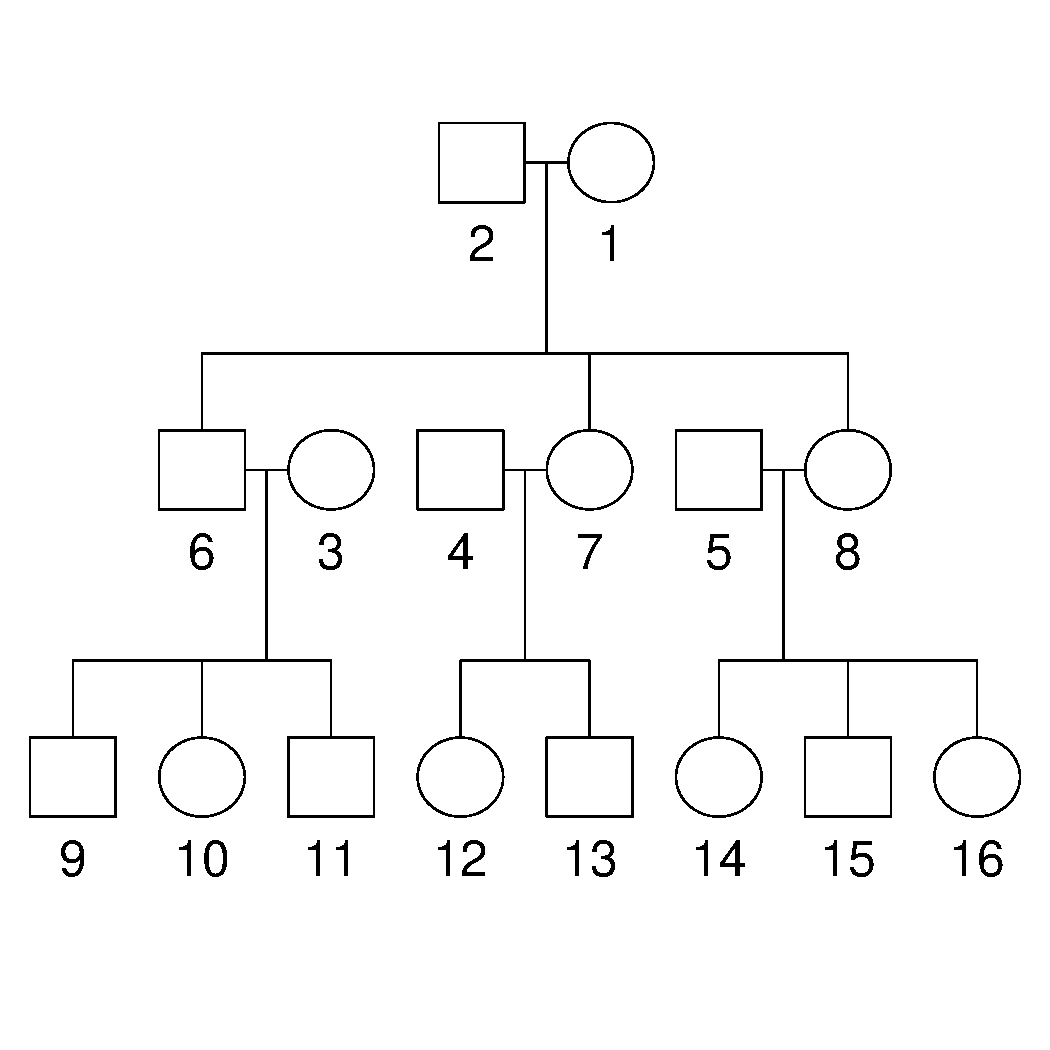
\includegraphics[height=7cm]{pedigree_16individs.pdf}
\caption{The 16-person pedigree used for the simulations.}
\label{ped}
\end{figure}

The full model assumed when testing for association on X chromosome SNPs (and one of the models used for simulating the X chromosome quantative phenotype) is 
\begin{align}
y &= \beta_0 + \beta_1 \snpX + g_A + g_X +\epsilon \\
g_A &\sim MVN(0,\sigma^2_A \Phi_A) \\
g_X &\sim MVN(0,\sigma^2_X \Phi_X) \\
\epsilon &\sim N(0,\sigma^2_\epsilon)
\end{align}
where SNP$_x$ is the vector of genotypes on the X chromosome SNP that is being tested for association, $\Phi_A$ is the matrix of kinship coefficients as measured on the autosomes and $\Phi_X$ is the matrix of X chromosome specific kinship coefficients. The male X chromosome genotypes are coded as 0, 2 and the female genotypes are coded as 0, 1, 2.

We calculate the variance for a given individual $i$ to be the sum of the variance of the SNP being tested, and the variances due to X chromosome, autosomal and other effects as
\begin{align}
var(y_i)&=\beta_1^2 var(\snpX)+\sigma^2_X +\sigma^2_A + \sigma^2_\epsilon
\end{align}

The variance of an X chromosome SNP can be calculated conditionally based on whether the sample is female or male. 
\begin{align}
\mathbb{E}(\snpXF)&=2p^2+2p(1-p)= 2p\\
\mathbb{E}(\snpXM)&=2p
\end{align} when the male genotypes are coded as 0, 2 and the female genotypes are coded as 0, 1, 2.
Then, we find that
\begin{align}
var(\snpXF)&= \mathbb{E}((\snpXF)^2)-\mathbb{E}^2(\snpX)\\
&=4p^2+2p(1-p)-(2p)^2\\ \label{fem_var}
&=2p(1-p)\\ 
var(\snpXM)&=\mathbb{E}((\snpXM)^2)-\mathbb{E}^2(\snpXM)\\
&=4p-(2p)^2\\
&=4p(1-p) \label{mal_var}
\end{align} 

To calculate the covariance of genotypes between a pair of individuals, we must consider their sex. In what follows, I am denoting the X chromosome kinship value between a pair of individuals as $\Phi_X$. Technically, this should be written as $\Phi_{X, ij}$ where $ij$ indexes the individuals $i$ and $j$ for which the X chromosome kinship value represents.
First, we calculate the covariance for a SNP between a pair of males as
\begin{align}
cov(\snpXM, \snpXM) &= \mathbb{E}(\snpXM \snpXM) - \mathbb{E}^2(\snpXM) \\
&=  \mathbb{E}(\snpXM \snpXM|\mbox{IBD})\mathbb{P}(\mbox{IBD}) \\
&\mbox{     }+\mathbb{E}(\snpXM \snpXM|\mbox{no IBD})\mathbb{P}(\mbox{no IBD})  -(2p)^2\\
&= \mathbb{E}(\snpXM \snpXM|\mbox{IBD})\Phi_X \\
&\mbox{     }  +\mathbb{E}(\snpXM \snpXM|\mbox{no IBD})(1-\Phi_X)-4p^2\\
&= 4p\Phi_X+4p^2(1-\Phi_X)-4p^2\\
&= 4p(1-p)\Phi_X
\end{align}
Next we consider the covariance between a pair of female genotypes
\begin{align}
cov(\snpXF,\snpXF) &= \mathbb{E}(\snpXF \snpXF) - \mathbb{E}^2(\snpXF) \\
&=  \mathbb{E}(\snpXF \snpXF|\mbox{IBD})\mathbb{P}(\mbox{IBD}) \\
&\mbox{     }+\mathbb{E}(\snpXF \snpXF|\mbox{no IBD})\mathbb{P}(\mbox{no IBD})  -(2p)^2\\
&= (2(2p(1-p))+4p^2)\Phi_X+4p^2(1-\Phi_X)-4p^2\\
&= 4p(1-p)\Phi_X
\end{align}
Finally, we calculate the covariance between a pair of genotypes where one is a female and one is a male
\begin{align}
cov(\snpXF,\snpXM) &= \mathbb{E}(\snpXF \snpXM) -\mathbb{E}(\snpXF)\mathbb{E}(\snpXM)\\
 &=  \mathbb{E}(\snpXF \snpXM|\mbox{IBD})\mathbb{P}(\mbox{IBD}) \\
&\mbox{     }+\mathbb{E}(\snpXF \snpXM|\mbox{no IBD})\mathbb{P}(\mbox{no IBD})  -(2p)^2\\
&= (4p^2+2(2p(1-p)))\Phi_X+4p^2(1-\Phi_X)-4p^2\\
&= 4p(1-p)\Phi_X
\end{align}
We can now see that using the X chromosome kinship values from Table~\ref{kc_auto_x}, the variance for a female and male SNP is indeed as calculated in Equations~\ref{fem_var} and~\ref{mal_var} after incorporating the self-kinship values. 
Thus, the variance for a given individual $i$ for an X chromosome SNP is 
\begin{align}
var(y_i)&=\beta_1^2 4p(1-p)\Phi_X+\sigma^2_X +\sigma^2_A + \sigma^2_\epsilon
\end{align}

The parameter $h^2_{snp}$ indicates the heritability of the X chromosome SNP. It can be calculated from the equation
\begin{align}
h^2_{snp}&=\frac{\beta_1^2 4p(1-p)\Phi_X}{\beta_1^2 4p(1-p)\Phi_X+\sigma^2_\epsilon + \sigma^2_A + \sigma^2_X}
\end{align}
where $p$ is the allele frequency of the causal SNP.
On the other hand, we can calculate the heritability of all SNPs on the X chromosome, which is 
\begin{align}
h^2_{x}&=\frac{\beta_1^2 4p(1-p)\Phi_X+\sigma^2_X}{\beta_1^2 4p(1-p)\Phi_X+\sigma^2_\epsilon + \sigma^2_A + \sigma^2_X}
\end{align}


%%%%%
\section*{Relatedness Estimation Using X Chromosome SNPs}

For the proposed model to work, we first must convince ourselves that we can accurately estimate relatedness using genetic material from the X chromosome. 
Table~\ref{kc_auto_x} displays the autosomal and X chromosome kinship coefficients (KC) for a given pair of relatives. The autosomal KC is defined as the probability of sampling two alleles IBD from a given pair of individuals. The X chromosome KC, on the other hand, is defined as the probability of sampling one allele IBD from an X chromosome in a given pair of individuals. Thus, the X chromosome KC will differ from the usual autosomal KC. Furthermore, when calculating the theoretical X chromosome KC, we must take into account the sex of the individuals, whether the pair is related maternally or paternally, and the type of relationship.

X chromosome relatedness can be estimated between two individuals using SNP genotypes. Let $j, k, l, m$ be four individuals such that $j, k$ are male and $l, m$ are female. The genotypes for each of the independent X chromosome SNPs in individual $j$ are denoted by $X_{ij}$ for SNPs $i \in \{1,\dots,N\}$ and are coded as 0, 1, 2 in females and 0, 2 in males.
We can estimate the genetic relatedness (GR) using SNP genotypes, which is twice the X chromsome KC in female-female pairs, $\sqrt{2}$ the X chromosome KC in female-male pairs and equal to the X chromosome KC in male-male pairs.
The X chromosome genetic relatedness between two individuals is
\begin{align}
\mbox{GR}_{FF}&=\frac{1}{N}\sum_{i=1}^N \frac{(X_{il}-2p_i)(X_{im}-2p_i)}{2p_i(1-p_i)}\\
\mbox{GR}_{MM}&=\frac{1}{N}\sum_{i=1}^N \frac{(X_{ij}-p_i)(X_{ik}-p_i)}{p_i(1-p_i)}\\
\mbox{GR}_{MF}&=\frac{1}{N}\sum_{i=1}^N \frac{(X_{ij}-p_i)(X_{il}-2p_i)}{\sqrt{2}p_i(1-p_i)}
\end{align}

To investigate how accurate we can estimate the X chromosome KC, I simulated varying numbers of X chromosome SNPs for one iteration of the 16-sample pedigree shown in Figure~\ref{ped}. The allele frequency of the SNPs was set at 0.4. Figure~\ref{xchr_relatedness} shows the difference between the estimated and theoretical X chromosome KC for all sample pairs for increasing numbers of SNPs.  Figures~\ref{xchr_relatedness_M},~\ref{xchr_relatedness_F} and~\ref{xchr_relatedness_MF} show the results broken up by the composition of sex in the related pair. 
Figure~\ref{xchr_hists} shows a histogram of the estimated X chromosome KC for each relationship type. The true value is shown with a red dotted line and the number of relationships at a given KC value is displayed in the plot title. Many of the relationships have a small sample size.  Some relationships are underestimated but all are generally centered around the truth.

As expected, with a larger number of SNPs, we are able to more accurately estimate the true X chromosome KC. We note from all Figures that the estimated KC is at most 0.06 away from the true value. The OLGA genotyping set resulted in approximately 3,500 SNPs on the X chromosome after pruning. Perhaps this number of SNPs, shown in orange in the Figures, should be considered most realistic. We conclude that we are sufficiently able to estimate the X chromosome KC from 3,500 independent, genotyped X chromosome SNPs.

\begin{figure}
\begin{center}
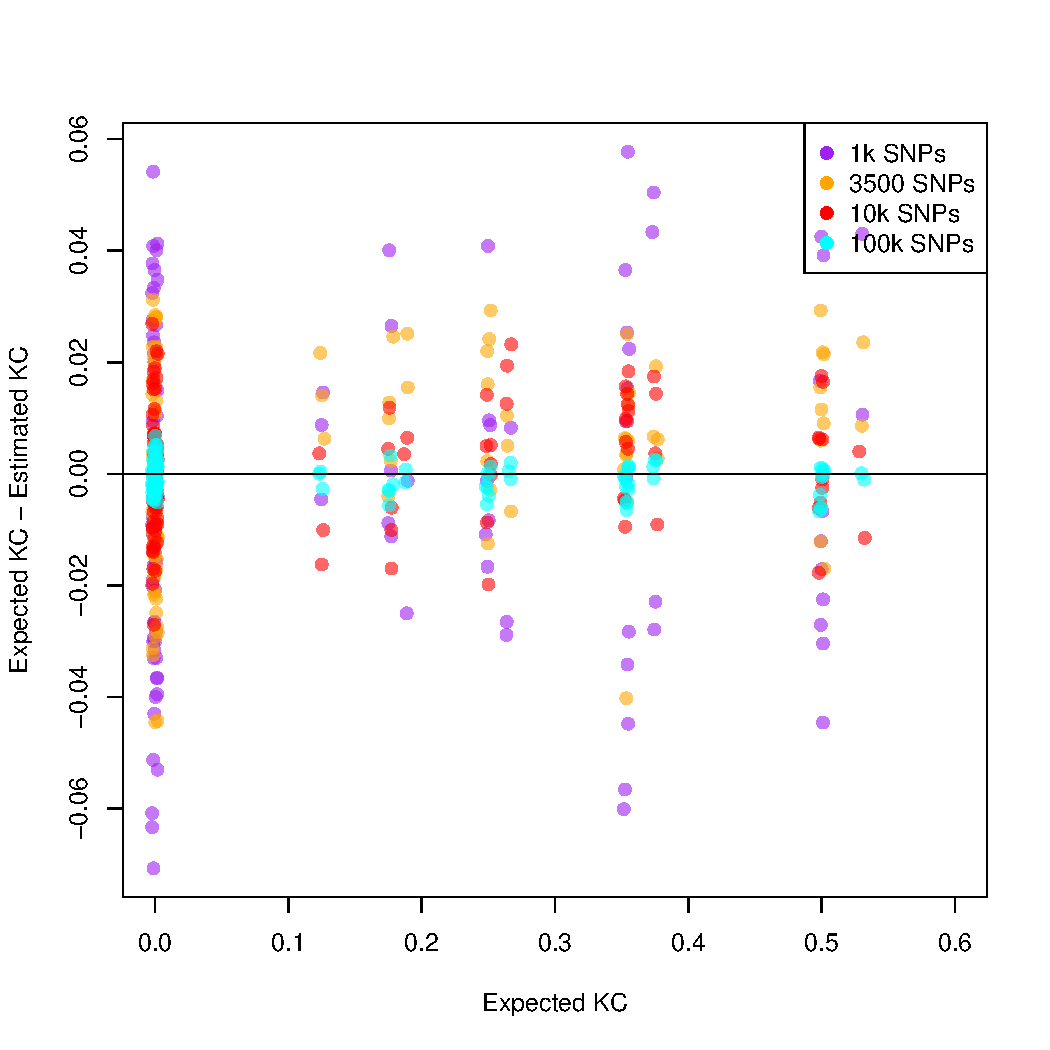
\includegraphics[height=3in]{xchrKcEstimatedVsTrue.pdf}
\caption{The expected X chromosome KC versus the difference between the expected and estimated X chromosome KC, for all sample pairs in the 16-person pedigree shown in Figure~\ref{ped}. The colors indicate the number of simulated X chromosome SNPs used to estimate the KC.}
\label{xchr_relatedness}
\end{center}
\end{figure}

\begin{figure}
\begin{center}
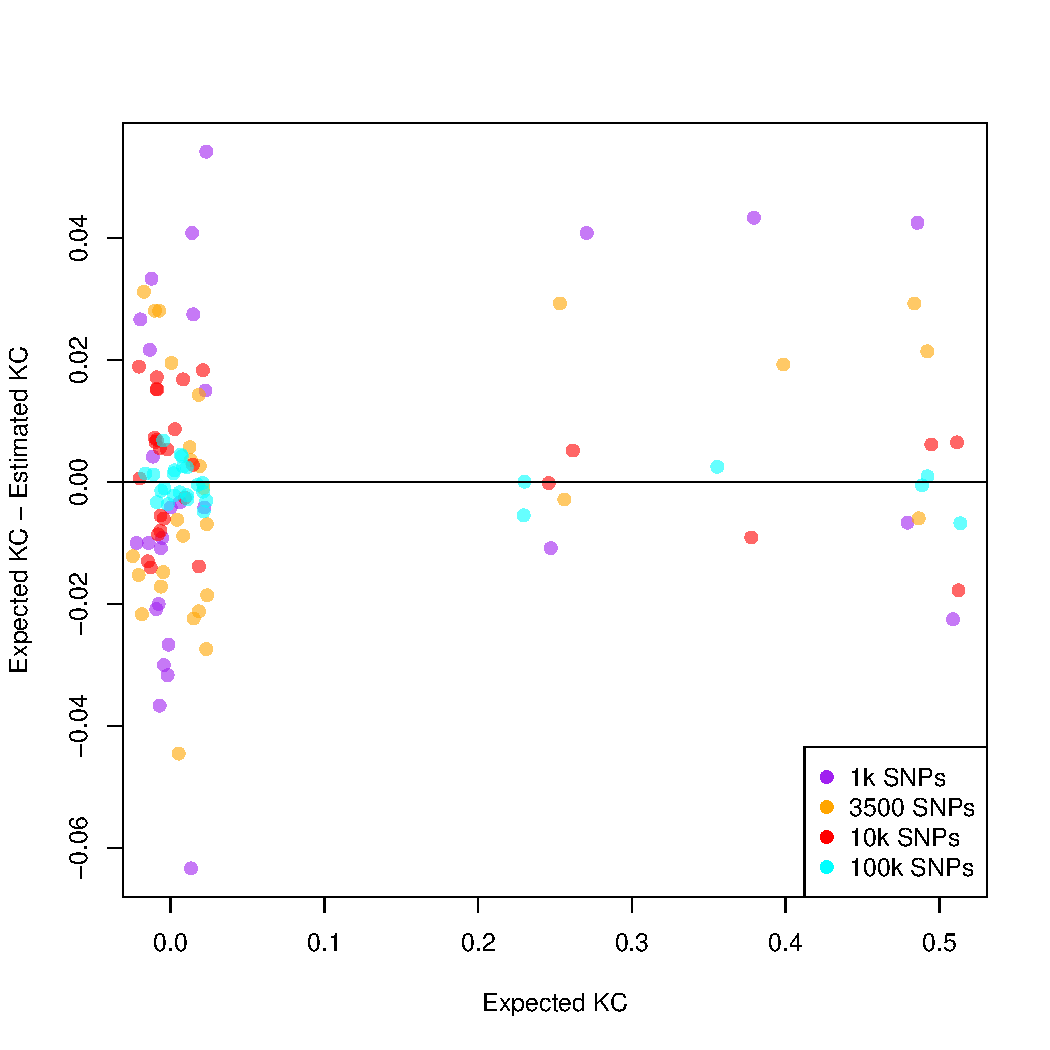
\includegraphics[height=3in]{xchrKcEstimatedVsTrueMM.pdf}
\caption{The expected X chromosome KC versus the difference between the expected and estimated X chromosome KC, for all male-male sample pairs in the 16-person pedigree shown in Figure~\ref{ped}. The colors indicate the number of simulated X chromosome SNPs used to estimate the KC.}
\label{xchr_relatedness_M}
\end{center}
\end{figure}

\begin{figure}
\begin{center}
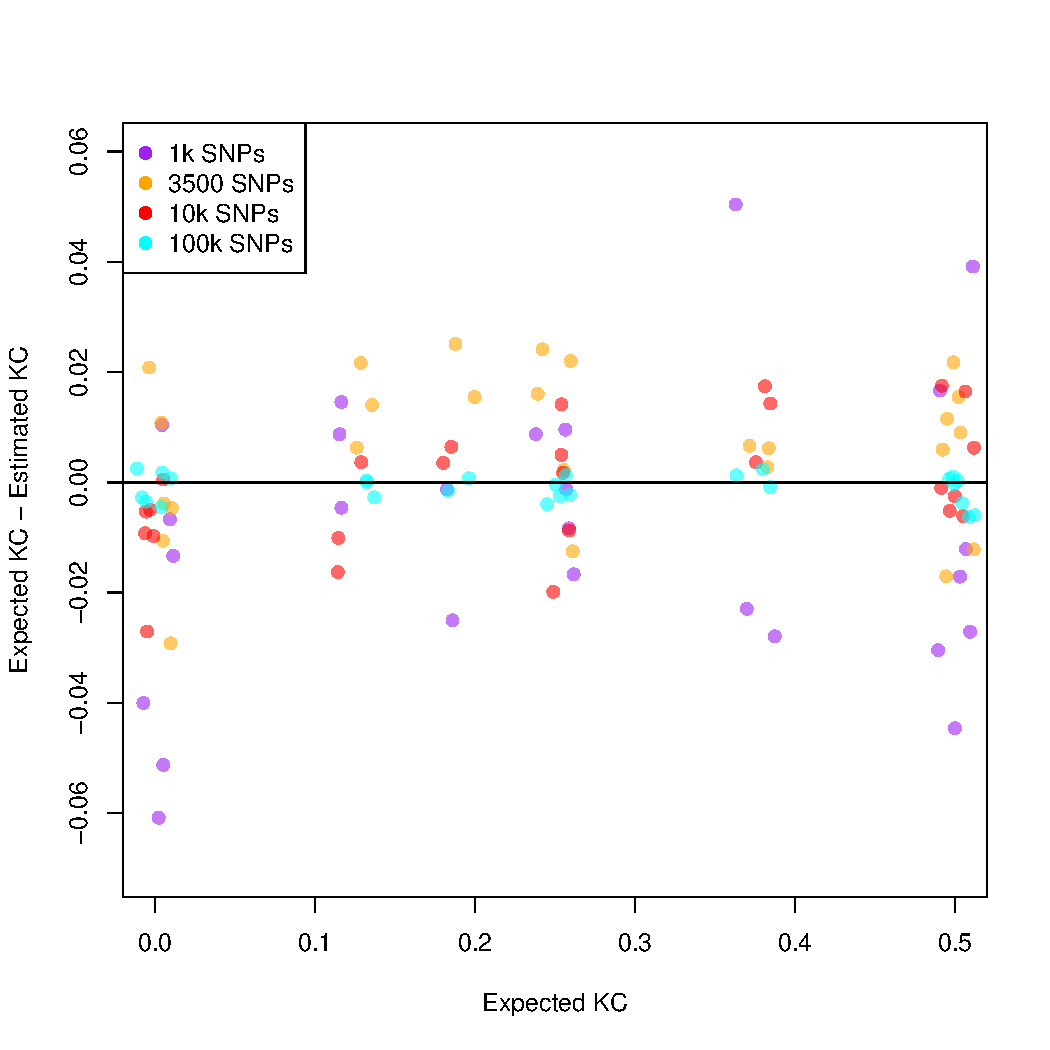
\includegraphics[height=3in]{xchrKcEstimatedVsTrueFF.pdf}
\caption{The expected X chromosome KC versus the difference between the expected and estimated X chromosome KC, for all female-female sample pairs in the 16-person pedigree shown in Figure~\ref{ped}. The colors indicate the number of simulated X chromosome SNPs used to estimate the KC.}
\label{xchr_relatedness_F}
\end{center}
\end{figure}

\begin{figure}
\begin{center}
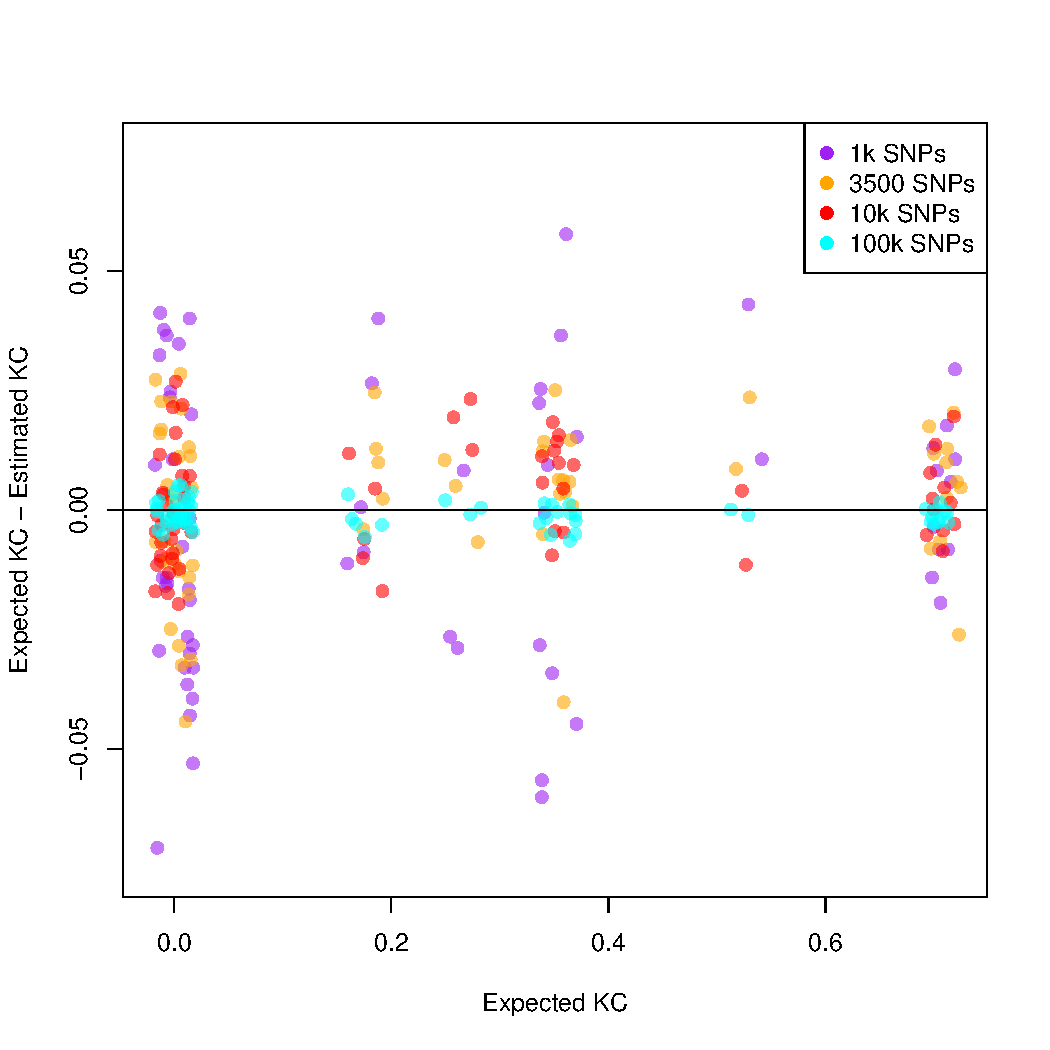
\includegraphics[height=3in]{xchrKcEstimatedVsTrueFM.pdf}
\caption{The expected X chromosome KC versus the difference between the expected and estimated X chromosome KC, for all female-male sample pairs in the 16-person pedigree shown in Figure~\ref{ped}. The colors indicate the number of simulated X chromosome SNPs used to estimate the KC.}
\label{xchr_relatedness_MF}
\end{center}
\end{figure}

\begin{figure}
\begin{center}
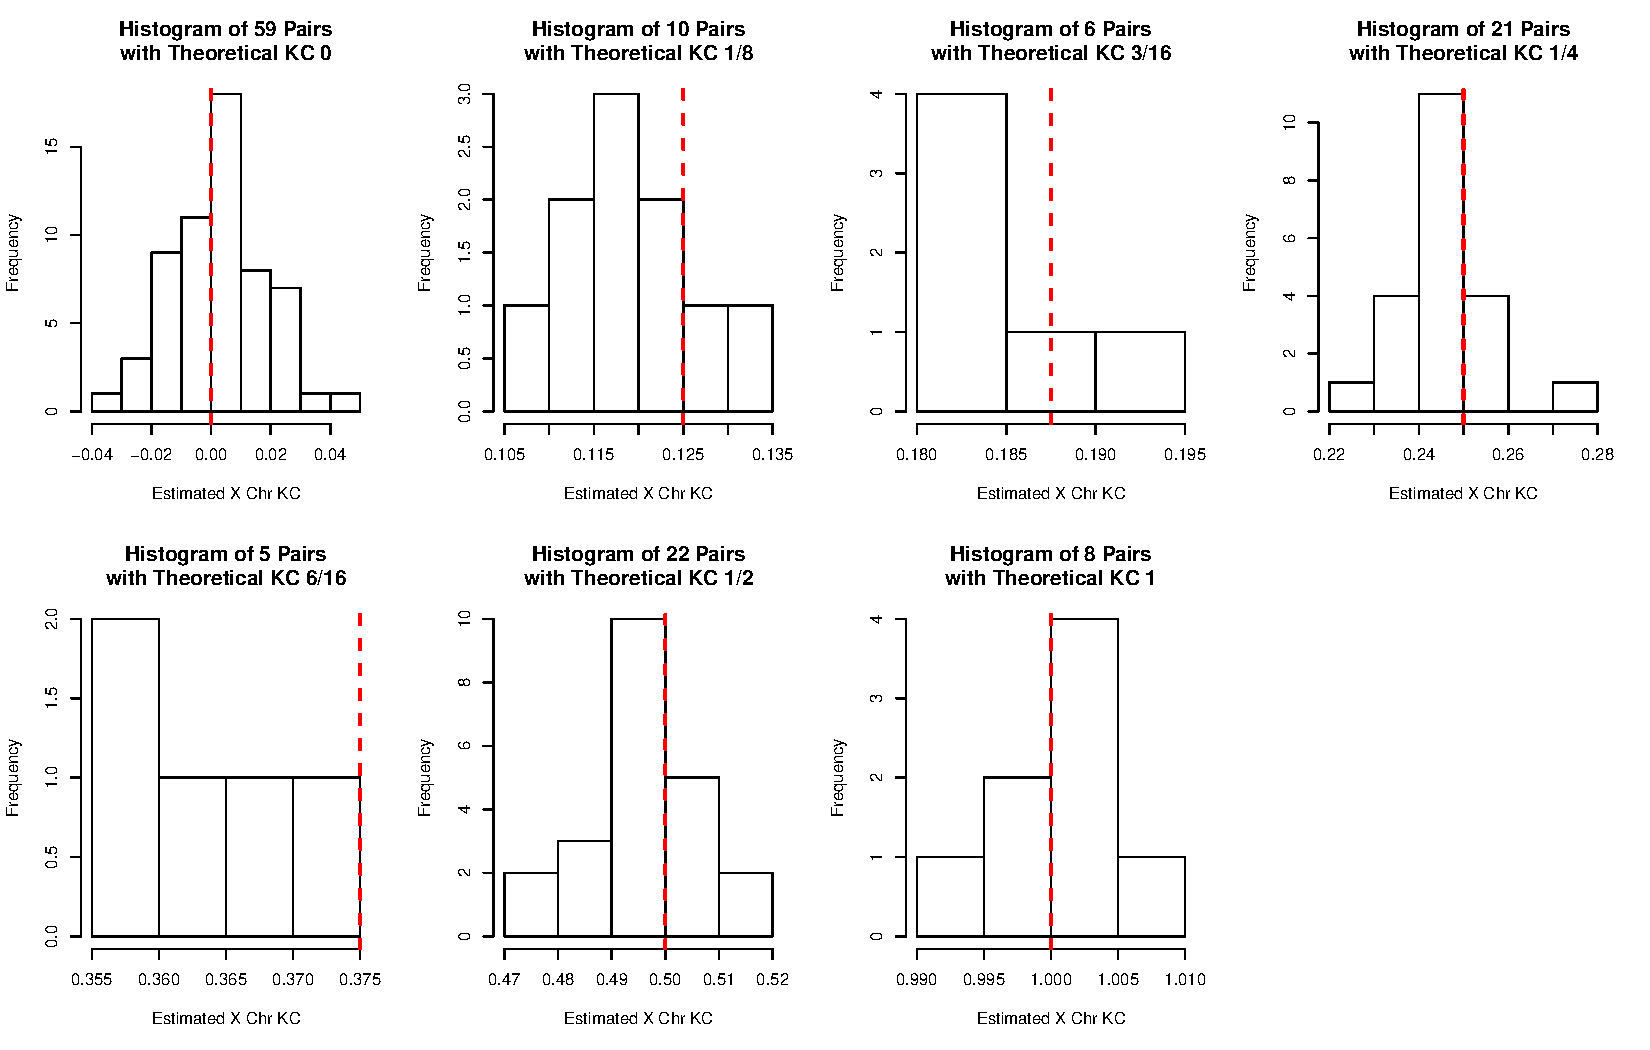
\includegraphics[height=4in]{histXchrKCByRelType.pdf}
\caption{Histograms of the estimated X chromosome KC, by relationship type, for all pairs of relatives shown in the pedigree in Figure~\ref{ped}. The true value is shown with a red dotted line. The estimates were calculated from 3,500 simulated SNPs.}
\label{xchr_hists}
\end{center}
\end{figure}




%%%%%
\section*{Variance Components Estimation}
I estimated the variance components for the autosomes, the X chromosome, and the remaining effects, using the true kinship matrix in both cases.
I then fit the mixed model for a quantitative trait on the X chromosome, testing the genotypes simulated on the X chromosome.

Initially, I investigated whether the estimated variance components were converging to what I expected. 
I simulated 10,000 independent pedigrees as shown in Figure~\ref{ped} for a total of 16,000 individuals, of whom 5,000 are unrelated (5 founders per pedigree), and performed this simulation 500 times. The relatedness matrices used were the true values, not the estimated ones. I estimated variance components for three models (where the phenotype was simulated from the given model): 
\begin{align}
\label{model1} y&=\beta_1 \snpX +\epsilon \\
\label{model2} y&=\beta_1 \snpX + g_X + \epsilon\\
\label{model3} y&=\beta_1 \snpX + g_X + g_A + \epsilon 
\end{align} with the specifications of 
\begin{align*}
g_A &\sim MVN(0,0.3 \Phi_A) \\
g_X &\sim MVN(0,0.8 \Phi_X) \\
\epsilon &\sim N(0,1)\\
\beta_1 &= 0.8 \\
p&=0.2
\end{align*}
From computations as shown above, in each of the three models we expect the estimates for $\sigma^2_X$,  $\sigma^2_A$ and $\sigma^2_\epsilon$ to be as displayed in Table~\ref{simMetrics} where $\sigma^2_{XT} = \beta_1^2 4 p(1-p) + \sigma_X^2$.
Table~\ref{varComp_sim_results} shows the results from the described simulation study. The standard deviations shown there are the mean lower and upper bounds as provided from Matt's confidence intervals, i.e. the confidence intervals calculated from each of the 500 iterations. We note that the simulations yield a mean value that is equal to the expected value. We conclude the variance components are being estimated accurately.

\bgroup
\def\arraystretch{1.5}
\begin{table}[ht]
\centering
\begin{tabular}{crrr}
  \hline
 Model & $\sigma^2_{XT}$ &  $\sigma^2_A$& $\sigma^2_\epsilon$  \\ 
  \hline
1 & 0.4096& -  & 1  \\
2 &1.2096& - & 1 \\
3 & 1.2096 & 0.3 & 1\\ 
   \hline
\end{tabular} 
\caption{Values of simulated variance components.}\label{simMetrics}
\end{table} 

\bgroup
\def\arraystretch{1.5}
\begin{table}[ht]
\centering
\begin{tabular}{crrr}
  \hline
 Model & $\sigma^2_{XT}$ &  $\sigma^2_A$& $\sigma^2_\epsilon$  \\ 
  \hline
1 & 0.4098 (0.3667, 0.4529)& -  & 1.001 (0.9685, 1.033)  \\
2 &1.210 (1.136, 1.284)& - & 0.9995 (0.9623, 1.037) \\
3 & 1.211 (1.103, 1.319) & 0.3035 (0.1303, 0.4768) & 1.000 (0.9525, 1.048)\\ 
   \hline
\end{tabular}
\caption{Mean (mean CI bounds) from simulation results for three models, where the variance components were simulated as shown in Table~\ref{simMetrics}. The simulation included 16,000 samples, of which 5,000 were unrelated.} \label{varComp_sim_results}
\end{table}



%%%%%
\section*{Association Testing on the X Chromosome}
I estimated the variance components for the autosomes, the X chromosome, and the remaining effects, using the known, theoretical autosomal and X chromosome kinship matrices.
I fit the mixed model for a quantitative trait on the X chromosome, testing the genotypes simulated on the X chromosome.

We can evaluate the type I error and power when the true model is 
\begin{align}
 y&=\beta_1 \snpX + g_X + g_A + \epsilon 
\end{align}
and when fitting the misspecified, usual model, $y=\beta_1 \snpX + g_A + \epsilon$. I also fit the 
misspecified model $y=\beta_1 \snpX + g_X + \epsilon$ for comparison.
From 1,000 iterations using 8,000 samples (500 pedigrees as displayed in Figure~\ref{ped}) of which 5,500 are related and 2,500 are unrelated, we set the 
parameters as shown in Table~\ref{params_sim}.
Because the usual model is not properly calibrated, we compare the false positive rate to the true positive rate.
In this manner, we can identify how many true positives (the power) we are able to detect for a given false positive rate (type I error). 

\begin{table}[ht]
\centering
\begin{tabular}{crrr}
\hline
Parameter & Sim1 & Sim2&Sim3\\ \hline
$\beta_1$& 0.8 &  0.3& 0.3\\ 
$\sigma_A^2$&0.3& 0.3& 0.3\\
$\sigma_X^2$&0.8 & 0.8& 0.3\\
$\sigma_{\epsilon}^2$&1& 1& 1\\\hline
$\sigma_{XT}^2$ & 1.2096& 0.8576& 0.3576\\ \hline
\end{tabular}
\caption{Parameters used in simulations.}
\label{params_sim}
\end{table} 
When the effect size reaches 0.18, all three models tested always found the true signal.
Plots showing the 
The type I error, however, differed in each of the models. Table~\ref{typeIerror} shows the type I errors when fitting the two models.

\bgroup
\def\arraystretch{1.5}
\begin{table}[ht]
\centering
\begin{tabular}{r|rrrrr}
  \hline
$\alpha$& 0.05 & 0.01 & 0.005 & 0.001 & 0.0001 \\ \hline
X + Auto adj & 0.04604 & 0.00834 & 0.00450 & 0.00092 & 0 \\ 
  Auto adj only & 0.06823 & 0.01960 & 0.01034 & 0.00133 & 0 \\ 
X chr adj only & 0.04446 & 0.00817 & 0.00509 & 0.00100 & 0 \\
   \hline
\end{tabular}
\caption{Type I error from 12,000 iterations of an 8,000 sample simulation. The true model is as described in Equation~\ref{model3} and the results are shown from fitting the true model, the model without fitting X chromosome effects, $y=\beta_1 \snpX + g_A + \epsilon$, and the model fitting only X chromosome effects $y=\beta_1 \snpX + g_X + \epsilon$.}\label{typeIerror}
\end{table} 


\begin{table}[ht]
\centering \small
\begin{tabular}{l|lll}
  \hline
 $\alpha$ & Auto + X & X & Auto \\ 
  \hline
0.05 (0.0496, 0.0504) & 0.04604 (0.04214, 0.04994) & 0.04446 (0.04056, 0.04836) & 0.06823 (0.06433, 0.07213) \\ 
0.01 (0.00960, 0.0104) & 0.00834 (0.00656, 0.01012) & 0.00817 (0.00639, 0.00996) & 0.01960 (0.01782, 0.02138) \\ 
0.005 (0.00460, 0.0054) & 0.00450 (0.00324, 0.00577) & 0.00509 (0.00383, 0.00635) & 0.01034 (0.00908, 0.01161) \\ 
0.001 (6.00e-04, 0.0014) & 0.00092 (0.00035, 0.00148) & 0.00100 (0.00044, 0.00157) & 0.00133 (0.00077, 0.00190) \\ 
 5e-04 (9.98e-05, 0.0009) & 0 (-0.00040, 0.00040) & 0.00017 (-0.00023, 0.00057) & 0 (-0.00040, 0.00040) \\ 
   \hline
\end{tabular}
\end{table}



%The genetic relatedness (GR) values were calculated using equations presented in (GCTA software paper) and are the following:
%\begin{align}
%GR(X_j,X_k)&=\frac{1}{N}\sum^N_i \frac{(X_{ij}-2p_i)(X_{ik}-2p_i)}{2p_i(1-p_i)} \\
%GR(X_j,X_l)&=\frac{1}{N}\sum^N_i \frac{(X_{ij}-2p_i)(X_{il}-p_i)}{\sqrt{2}p_i(1-p_i)}\\
%GR(X_l,X_m)&=\frac{1}{N}\sum^N_i \frac{(X_{il}-p_i)(X_{im}-p_i)}{p_i(1-p_i)}
%\end{align}
%where $X_j$ and $X_k$ are females and $X_l$ and $X_m$ are males.
%
%\bgroup
%\def\arraystretch{1.5}
%\begin{table}[ht]
%\centering
%\begin{tabular}{crcc}
%  \hline
%&& Autosomes & X Chromosome\\
%  \hline
%&Mother-Daughter &$\frac{1}{2}$ & $\frac{1}{2}$\\
%&Mother-Son, Father-Daughter &$\frac{1}{2}$& $\frac{\sqrt{2}}{2}$\\
%%&Father-Daughter &$\frac{1}{2}$&$\frac{\sqrt{2}}{2}$\\
%&Father-Son &$\frac{1}{2}$&0\\
%&Full sisters & $\frac{1}{2}$ & $\frac{3}{4}$\\
%&Full brothers &$\frac{1}{2}$&$\frac{1}{2}$\\
%&Sister-Brother &$\frac{1}{2}$&$\frac{\sqrt{2}}{4}$\\
%\hline
%\parbox[t]{2mm}{\multirow{8}{*}{\rotatebox[origin=c]{90}{\Large{Maternal}}}} & Aunt-Niece &$\frac{1}{4}$&$\frac{6}{16}$\\
%&Aunt-Nephew&$\frac{1}{4}$&$\frac{3\sqrt{2}}{8}$\\
%&Uncle-Niece &$\frac{1}{4}$&$\frac{\sqrt{2}}{8}$\\
%&Uncle-Nephew &$\frac{1}{4}$&$\frac{1}{4}$\\
%&Grandma-Granddaughter &$\frac{1}{4}$&$\frac{1}{4}$\\
%&Grandma-Grandson &$\frac{1}{4}$&$\frac{\sqrt{2}}{4}$\\
%&Grandpa-Granddaughter&$\frac{1}{4}$&$\frac{\sqrt{2}}{4}$\\
%&Grandpa-Grandson &$\frac{1}{4}$&$\frac{1}{2}$\\
%\hline
%\parbox[t]{2mm}{\multirow{8}{*}{\rotatebox[origin=c]{90}{\Large{Paternal}}}} &Aunt-Niece &$\frac{1}{4}$&$\frac{1}{4}$\\
%&Aunt-Nephew&$\frac{1}{4}$&0\\
%&Uncle-Niece &$\frac{1}{4}$&0\\
%&Uncle-Nephew &$\frac{1}{4}$&0\\
%&Grandma-Granddaughter &$\frac{1}{4}$&$\frac{1}{2}$\\
%&Grandma-Grandson &$\frac{1}{4}$&0\\
%&Grandpa-Granddaughter&$\frac{1}{4}$&0\\
%&Grandpa-Grandson &$\frac{1}{4}$&0\\
%   \hline
%\end{tabular}
%\caption{The theoretical genetic relatedness (GR) values stratified by X chromosome and autosomes. The autosomal GR value is twice the kinship coefficient $= 2(\frac{1}{2}\kappa_2+\frac{1}{4}\kappa_1)$, where $\kappa_1$ and $\kappa_2$ are the probabilities of sampling one and two alleles IBD, respectively. The X chromosome GR value for male-male pairs is $\kappa_1$, the probability of sampling one allele IBD. Female-female pairs yield an X chromosome GR value of twice $\kappa_1$ as calculated on the X chromosome. For female-male pairs, the X chromosome GR value is $\sqrt{2}\kappa_1$.}
%\end{table}



\bgroup
\def\arraystretch{1.5}
\begin{table}[ht]
\small
\centering
\begin{tabular}{crcc}
  \hline
&& Autosomes & X Chromosome\\
  \hline
& Self, Female & $\frac{1}{2}$ & $\frac{1}{2}$ \\
& Self, Male & $\frac{1}{2}$ & $1$ \\ \hline
&Mother-Daughter &$\frac{1}{4}$ & $\frac{1}{4}$\\
&Mother-Son, Father-Daughter &$\frac{1}{4}$& $\frac{1}{2}$\\
&Father-Son &$\frac{1}{4}$&0\\
&Full sisters & $\frac{1}{4}$ & $\frac{6}{16}$\\
&Full brothers &$\frac{1}{4}$&$\frac{1}{2}$\\
&Sister-Brother &$\frac{1}{4}$&$\frac{1}{4}$\\
\hline
\parbox[t]{2mm}{\multirow{8}{*}{\rotatebox[origin=c]{90}{\Large{Maternal}}}} & Aunt-Niece &$\frac{1}{8}$&$\frac{3}{16}$\\
&Aunt-Nephew&$\frac{1}{8}$&$\frac{6}{16}$\\
&Uncle-Niece &$\frac{1}{8}$&$\frac{1}{8}$\\
&Uncle-Nephew &$\frac{1}{8}$&$\frac{1}{4}$\\
&Grandma-Granddaughter &$\frac{1}{8}$&$\frac{1}{8}$\\
&Grandma-Grandson &$\frac{1}{8}$&$\frac{1}{4}$\\
&Grandpa-Granddaughter&$\frac{1}{8}$&$\frac{1}{4}$\\
&Grandpa-Grandson &$\frac{1}{8}$&$\frac{1}{2}$\\
\hline
\parbox[t]{2mm}{\multirow{8}{*}{\rotatebox[origin=c]{90}{\Large{Paternal}}}} &Aunt-Niece &$\frac{1}{8}$&$\frac{1}{8}$\\
&Aunt-Nephew&$\frac{1}{8}$&0\\
&Uncle-Niece &$\frac{1}{8}$&0\\
&Uncle-Nephew &$\frac{1}{8}$&0\\
&Grandma-Granddaughter &$\frac{1}{8}$&$\frac{1}{4}$\\
&Grandma-Grandson &$\frac{1}{8}$&0\\
&Grandpa-Granddaughter&$\frac{1}{8}$&0\\
&Grandpa-Grandson &$\frac{1}{8}$&0\\
   \hline \hline
Maternal-Maternal & First cousins, Girl-Girl & $\frac{1}{16}$ & $\frac{3}{32}$\\
& First cousins, Girl-Boy & $\frac{1}{16}$ & $\frac{3}{16}$\\
& First cousins, Boy-Boy & $\frac{1}{16}$ & $\frac{6}{16}$\\
\hline
Paternal-Paternal & First cousins, Girl-Girl & $\frac{1}{16}$ & $\frac{1}{32}$\\
& First cousins, Girl-Boy & $\frac{1}{16}$ & 0\\
& First cousins, Boy-Boy & $\frac{1}{16}$ & 0\\
\hline
Paternal-Maternal & First cousins, Girl-Girl & $\frac{1}{16}$ & $\frac{1}{16}$\\
& First cousins, Girl-Boy & $\frac{1}{16}$ & 0\\
& First cousins, Boy-Boy & $\frac{1}{16}$ & 0\\
\hline
\end{tabular}
\caption{The theoretical kinship coefficients (KC) stratified by X chromosome and autosomes. The autosomal KC value is $\frac{1}{2}\kappa_2+\frac{1}{4}\kappa_1$, where $\kappa_1$ and $\kappa_2$ are the probabilities of sampling one and two alleles IBD, respectively. The X chromosome KC value is the probability of sampling one allele IBD on the X chromosome in a given pair of individuals.}
\label{kc_auto_x}
\end{table}




\bgroup
\def\arraystretch{1.5}
\begin{table}[ht]
\small
\centering
\begin{tabular}{crcc}
  \hline
&& Autosomes & X Chromosome\\
  \hline
& Self, Male & $\frac{1}{2}$ & $1$ \\ \hline
& Self, Female & $\frac{1}{2}$ & $\frac{1}{2}$ \\
&Mother-Son, Father-Daughter &$\frac{1}{4}$& $\frac{1}{2}$\\
&Full brothers &$\frac{1}{4}$&$\frac{1}{2}$\\
Maternal&Grandpa-Grandson &$\frac{1}{8}$&$\frac{1}{2}$\\ \hline

&Full sisters & $\frac{1}{4}$ & $\frac{6}{16}$\\
Maternal&Aunt-Nephew&$\frac{1}{8}$&$\frac{6}{16}$\\ \hline


&Mother-Daughter &$\frac{1}{4}$ & $\frac{1}{4}$\\
&Sister-Brother &$\frac{1}{4}$&$\frac{1}{4}$\\
Maternal&Uncle-Nephew &$\frac{1}{8}$&$\frac{1}{4}$\\
Maternal&Grandma-Grandson &$\frac{1}{8}$&$\frac{1}{4}$\\
Maternal&Grandpa-Granddaughter&$\frac{1}{8}$&$\frac{1}{4}$\\
Paternal&Grandma-Granddaughter &$\frac{1}{8}$&$\frac{1}{4}$\\ \hline

Maternal& Aunt-Niece &$\frac{1}{8}$&$\frac{3}{16}$\\
Maternal-Maternal& First cousins, Girl-Boy & $\frac{1}{16}$ & $\frac{3}{16}$\\
Maternal-Maternal& First cousins, Boy-Boy & $\frac{1}{16}$ & $\frac{6}{16}$\\
 \hline

Maternal&Uncle-Niece &$\frac{1}{8}$&$\frac{1}{8}$\\
Maternal&Grandma-Granddaughter &$\frac{1}{8}$&$\frac{1}{8}$\\
Paternal&Aunt-Niece &$\frac{1}{8}$&$\frac{1}{8}$\\ \hline

Maternal-Maternal & First cousins, Girl-Girl & $\frac{1}{16}$ & $\frac{3}{32}$\\ \hline

Paternal-Maternal & First cousins, Girl-Girl & $\frac{1}{16}$ & $\frac{1}{16}$\\ \hline

Paternal-Paternal & First cousins, Girl-Girl & $\frac{1}{16}$ & $\frac{1}{32}$\\ \hline

&Father-Son &$\frac{1}{4}$&0\\
Paternal&Aunt-Nephew&$\frac{1}{8}$&0\\
Paternal&Uncle-Niece &$\frac{1}{8}$&0\\
Paternal&Uncle-Nephew &$\frac{1}{8}$&0\\
Paternal&Grandma-Grandson &$\frac{1}{8}$&0\\
Paternal&Grandpa-Granddaughter&$\frac{1}{8}$&0\\
Paternal&Grandpa-Grandson &$\frac{1}{8}$&0\\
Paternal-Paternal & First cousins, Girl-Boy & $\frac{1}{16}$ & 0\\
Paternal-Paternal & First cousins, Boy-Boy & $\frac{1}{16}$ & 0\\
Paternal-Maternal& First cousins, Girl-Boy & $\frac{1}{16}$ & 0\\
Paternal-Maternal& First cousins, Boy-Boy & $\frac{1}{16}$ & 0\\
\hline
\end{tabular}
\caption{The theoretical kinship coefficients (KC) stratified by X chromosome and autosomes. The autosomal KC value is $\frac{1}{2}\kappa_2+\frac{1}{4}\kappa_1$, where $\kappa_1$ and $\kappa_2$ are the probabilities of sampling one and two alleles IBD, respectively. The X chromosome KC value is the probability of sampling one allele IBD on the X chromosome in a given pair of individuals.}
\label{kc_auto_x_groupedByValue}
\end{table}




%
%\bgroup
%\def\arraystretch{1.0}
%\begin{table}[ht]
%\centering
%\begin{tabular}{r|rrrrr}
%  \hline
%Adjustment & $\alpha=0.01$ & $\alpha=0.005$ & $\alpha=0.001$ & $\alpha=5e-04$ & $\alpha=1e-04$ \\ 
%  \hline
% Auto & 0.01740 & 0.00968 & 0.00241 & 0.00137 & 0.00033 \\ 
%X & 0.01028 & 0.00521 & 0.00104 & 0.00053 & 0.00010 \\ 
%X + Auto & 0.01037 & 0.00513 & 0.00104 & 0.00053 & 0.00011 \\ 
%   \hline
%\end{tabular}
%\caption{Type I error for SNPs with varying minor allele frequencies. These were calculated from 839,760 iterations, where the correlation matrix for the autosomes was the KC matrix and the X chromosome-specific matrix was used for the X chromosome (see values in Table~\ref{kc_auto_x}).}
%\label{typeIvars}
%\end{table}
%
%\begin{table}[ht]
%\centering
%\begin{tabular}{r|rrrrr}
%  \hline
%Adjustment & $\alpha=0.01$ & $\alpha=0.005$ & $\alpha=0.001$ & $\alpha=5e-04$ & $\alpha=1e-04$ \\ 
%  \hline
%Auto & 0.01559 & 0.00849 & 0.00206 & 0.00112 & 0.00024 \\ 
%  X & 0.01046 & 0.00532 & 0.00110 & 0.00054 & 0.00011 \\ 
%  X + Auto & 0.01043 & 0.00528 & 0.00113 & 0.00055 & 0.00010 \\ 
%   \hline
%\end{tabular}
%\caption{Type I error for SNPs with varying minor allele frequencies. These were calculated from 839,760 iterations, where the correlation matrix for the autosomes was 2KC matrix and the X chromosome-specific matrix was adjusted to be 2KC, $\sqrt{2}$KC and KC for female-female, female-male and male-male pairs, respectively.}
%\label{typeIvars}
%\end{table}
%
%
%\begin{landscape}
%\begin{table}[ht]
%\centering
%\tiny
%\begin{tabular}{rrrrr|rrr|rrr|rrr|rrr|rrr}
%  \hline
%& & & & & \multicolumn{3}{c}{$\alpha=0.01$} & \multicolumn{3}{c}{$\alpha=0.005$} & \multicolumn{3}{c}{$\alpha=0.001$} & \multicolumn{3}{c}{$\alpha=5e-4$}&\multicolumn{3}{c}{$\alpha=1e-4$}\\
%$h_{x}$& $\beta_1$ & $h_{snp}$ & $\sigma^2_A$ & $\sigma^2_X$ & X & Auto & Both &X & Auto & Both & X &Auto & Both & X & Auto & Both & X & Auto & Both\\ 
%  \hline
% 0.1956 & 0.1835 & 0.010 & 0.3 & 0.3 & 356 & 454 & 360 & 186 & 252 & 188 & 36 & 61 & 41 & 16 & 29 & 18 & 7 & 7 & 6 \\ 
% 0.1514 & 0.2102 & 0.010 & 0.8 & 0.3 & 357 & 475 & 377 & 182 & 234 & 167 & 37 & 46 & 30 & 17 & 25 & 19 & 3 & 7 & 4 \\ 
% 0.3871 & 0.2102 & 0.010 & 0.3 & 0.8 & 392 & 627 & 382 & 201 & 377 & 202 & 47 & 98 & 47 & 25 & 64 & 26 & 7 & 19 & 6 \\ 
% 0.3146 & 0.2339 & 0.010 & 0.8 & 0.8 & 360 & 623 & 365 & 175 & 339 & 170 & 29 & 73 & 31 & 14 & 38 & 10 & 1 & 6 & 1 \\ 
% 0.2078 & 0.2924 & 0.025 & 0.3 & 0.3 & 346 & 466 & 353 & 168 & 232 & 171 & 33 & 47 & 32 & 18 & 25 & 18 & 3 & 8 & 5 \\ 
% 0.1643 & 0.3349 & 0.025 & 0.8 & 0.3 & 377 & 463 & 370 & 187 & 247 & 195 & 53 & 62 & 50 & 25 & 40 & 28 & 4 & 10 & 5 \\ 
% 0.3964 & 0.3349 & 0.025 & 0.3 & 0.8 & 374 & 628 & 379 & 200 & 366 & 202 & 39 & 90 & 38 & 15 & 54 & 18 & 2 & 10 & 2 \\ 
% 0.3250 & 0.3727 & 0.025 & 0.8 & 0.8 & 394 & 635 & 397 & 202 & 358 & 194 & 30 & 81 & 31 & 15 & 47 & 14 & 2 & 6 & 2 \\ 
%  0.2281 & 0.4189 & 0.050 & 0.3 & 0.3 & 342 & 483 & 346 & 165 & 260 & 160 & 41 & 64 & 41 & 28 & 45 & 26 & 10 & 16 & 11 \\ 
% 0.1857 & 0.4799 & 0.050 & 0.8 & 0.3 & 339 & 477 & 326 & 187 & 254 & 169 & 28 & 53 & 29 & 13 & 24 & 15 & 3 & 6 & 4 \\ 
% 0.4119 & 0.4799 & 0.050 & 0.3 & 0.8 & 348 & 600 & 339 & 167 & 328 & 162 & 34 & 78 & 33 & 14 & 45 & 12 & 4 & 9 & 4 \\ 
% 0.3423 & 0.5339 & 0.050 & 0.8 & 0.8 & 365 & 630 & 376 & 200 & 369 & 191 & 36 & 88 & 32 & 10 & 55 & 13 & 2 & 12 & 2 \\ 
% 0.2688 & 0.6086 & 0.100 & 0.3 & 0.3 & 355 & 506 & 365 & 167 & 275 & 169 & 37 & 58 & 37 & 18 & 32 & 20 & 3 & 8 & 3 \\ 
% 0.2286 & 0.6972 & 0.100 & 0.8 & 0.3 & 343 & 537 & 359 & 175 & 293 & 167 & 38 & 66 & 36 & 9 & 32 & 14 & 1 & 5 & 2 \\ 
% 0.4429 & 0.6972 & 0.100 & 0.3 & 0.8 & 322 & 681 & 326 & 154 & 389 & 159 & 29 & 98 & 28 & 18 & 52 & 15 & 1 & 9 & 1 \\ 
% 0.3769 & 0.7758 & 0.100 & 0.8 & 0.8 & 336 & 666 & 334 & 179 & 369 & 183 & 41 & 103 & 45 & 26 & 64 & 21 & 2 & 13 & 4 \\ 
% 0.3500 & 0.9129 & 0.200 & 0.3 & 0.3 & 364 & 606 & 365 & 187 & 310 & 183 & 31 & 79 & 29 & 12 & 41 & 10 & 2 & 8 & 3 \\ 
% 0.3143 & 1.0458 & 0.200 & 0.8 & 0.3 & 363 & 628 & 373 & 184 & 362 & 184 & 34 & 83 & 35 & 21 & 41 & 20 & 7 & 12 & 6 \\ 
% 0.5048 & 1.0458 & 0.200 & 0.3 & 0.8 & 349 & 760 & 357 & 179 & 428 & 177 & 40 & 119 & 39 & 18 & 70 & 19 & 2 & 19 & 2 \\ 
% 0.4462 & 1.1637 & 0.200 & 0.8 & 0.8 & 393 & 788 & 395 & 223 & 442 & 211 & 47 & 132 & 46 & 34 & 77 & 32 & 8 & 26 & 8 \\ 
% 0.3744 & 0.9978 & 0.230 & 0.3 & 0.3 & 373 & 636 & 381 & 170 & 356 & 171 & 35 & 95 & 40 & 21 & 57 & 21 & 3 & 15 & 2 \\ 
% 0.3400 & 1.1432 & 0.230 & 0.8 & 0.3 & 361 & 653 & 362 & 186 & 379 & 183 & 34 & 105 & 32 & 23 & 53 & 22 & 3 & 18 & 4 \\ 
% 0.5233 & 1.1432 & 0.230 & 0.3 & 0.8 & 381 & 858 & 372 & 190 & 487 & 192 & 36 & 141 & 35 & 18 & 79 & 17 & 4 & 18 & 4 \\ 
% 0.4669 & 1.2720 & 0.230 & 0.8 & 0.8 & 342 & 729 & 346 & 160 & 424 & 161 & 31 & 108 & 33 & 18 & 58 & 18 & 1 & 14 & 1 \\ 
%   \hline
%&\multicolumn{4}{r|}{Totals} &8632 & 14609 & 8705 & 4374 & 8130 & 4311 & 876 & 2028 & 870 & 446 & 1147 & 446 & 85 & 281 & 92 \\ \hline
% \multicolumn{5}{r|}{Type I Error Rates}& 0.01028 & 0.01740 & 0.01037 & 0.00521 & 0.00968 & 0.00513 & 0.00104 & 0.00241 & 0.00104 & 0.00053 & 0.00137 & 0.00053 & 0.00010 & 0.00033 & 0.00011 \\ 
%   \hline 
%\end{tabular}
%\caption{Counts of false postives for varying parameter values, stratified by adjustment for X relatedness, autosomal relatedness, and adjustment for both. In all simulations, $\sigma^2_\epsilon$ was set to 1 and $p$ was set to 0.2. There were 34,990 simulations performed at each parameter combination for a total of 839,760 simulations. Five values of $\alpha$ were considered, although the final two are quite small. The bottom row is the total number of false positives for each column and the corresponding type I error rates averaged across all parameter values considered. These are precisely the values shown in Table~\ref{typeIvars}.}
%\end{table}
%\end{landscape}
%
%
%\begin{table}[ht]
%\centering
%\begin{tabular}{rrrrr|rrr}
%  \hline
% & $\beta_1$ & $h^2$ & $p$ & $\sigma^2_X$ & $\sigma^2_{XT}$ & $\sigma^2_A$ & $\sigma^2_\epsilon$ \\ 
%  \hline
%1 & 0.1835 & 0.01 & 0.2 & 0.3 & 0.3162 & 0.3 & 1 \\ 
%  2 & 0.2102 & 0.01 & 0.2 & 0.3 & 0.3212 & 0.8 & 1 \\ 
%  3 & 0.2102 & 0.01 & 0.2 & 0.8 & 0.8212 & 0.3 & 1 \\ 
%  4 & 0.2339 & 0.01 & 0.2 & 0.8 & 0.8263 & 0.8 & 1 \\ 
%  5 & 0.2924 & 0.03 & 0.2 & 0.3 & 0.3410 & 0.3 & 1 \\ 
%  6 & 0.3349 & 0.03 & 0.2 & 0.3 & 0.3538 & 0.8 & 1 \\ 
%  7 & 0.3349 & 0.03 & 0.2 & 0.8 & 0.8538 & 0.3 & 1 \\ 
%  8 & 0.3727 & 0.03 & 0.2 & 0.8 & 0.8667 & 0.8 & 1 \\ 
%  9 & 0.4189 & 0.05 & 0.2 & 0.3 & 0.3842 & 0.3 & 1 \\ 
%  10 & 0.4799 & 0.05 & 0.2 & 0.3 & 0.4105 & 0.8 & 1 \\ 
%  11 & 0.4799 & 0.05 & 0.2 & 0.8 & 0.9105 & 0.3 & 1 \\ 
%  12 & 0.5339 & 0.05 & 0.2 & 0.8 & 0.9368 & 0.8 & 1 \\ 
%  13 & 0.6086 & 0.10 & 0.2 & 0.3 & 0.4778 & 0.3 & 1 \\ 
%  14 & 0.6972 & 0.10 & 0.2 & 0.3 & 0.5333 & 0.8 & 1 \\ 
%  15 & 0.6972 & 0.10 & 0.2 & 0.8 & 1.0333 & 0.3 & 1 \\ 
%  16 & 0.7758 & 0.10 & 0.2 & 0.8 & 1.0889 & 0.8 & 1 \\ 
%  17 & 0.9129 & 0.20 & 0.2 & 0.3 & 0.7000 & 0.3 & 1 \\ 
%  18 & 1.0458 & 0.20 & 0.2 & 0.3 & 0.8250 & 0.8 & 1 \\ 
%  19 & 1.0458 & 0.20 & 0.2 & 0.8 & 1.3250 & 0.3 & 1 \\ 
%  20 & 1.1637 & 0.20 & 0.2 & 0.8 & 1.4500 & 0.8 & 1 \\ 
%  21 & 0.9978 & 0.23 & 0.2 & 0.3 & 0.7779 & 0.3 & 1 \\ 
%  22 & 1.1432 & 0.23 & 0.2 & 0.3 & 0.9273 & 0.8 & 1 \\ 
%  23 & 1.1432 & 0.23 & 0.2 & 0.8 & 1.4273 & 0.3 & 1 \\ 
%  24 & 1.2720 & 0.23 & 0.2 & 0.8 & 1.5766 & 0.8 & 1 \\ 
%   \hline
%\end{tabular}
%\caption{Metrics used in the simulations, of which there were 24 combinations. These correspond to the 24 variance components results shown in Tables~\ref{varCompKC} and~\ref{varCompKC_mf}. Shown in the final 3 columns are the true variances that we aim to estimate.}
%\end{table}



\newpage
\textbf{Performing Mixed Model Association Testing on the X Chromosome}

To perform mixed model association testing on X chromsome SNPs, there are a few steps to take.
\begin{enumerate}
\item Estimate relatedness on the X chromosome, call the results $\Phi_X$. Use independent (pruned) SNPs, excluding the pseudoautosomal regions. In OLGA, the number of pruned X chromosome SNPs was approximately 3,500. Histograms of the results for theoretical vs estimated in 3,500 simulated X chromosome SNPs for the pedigree in Figure~\ref{ped} are shown in the file `hist\_xchrKC\_byRelType.pdf.' 
\item Run Matt's MLM program, including as a random effect the relatedness matrix on the X chromosome, $\Phi_X$. We are investigating the implications of including $\Phi_A$ as well, when testing a SNP on the X chromsome for association.
\end{enumerate}


\end{document}




